\documentclass[11pt]{article}

\usepackage[utf8]{inputenc}
\usepackage[T1]{fontenc}
\usepackage{amsmath,amssymb}
\usepackage{booktabs}
\usepackage{graphicx}
\usepackage{hyperref}
\usepackage{url}
\usepackage[margin=1in]{geometry}
\usepackage{authblk}

\title{Perplexity Holds, Programs Break:\\ Executable Correctness as a Blind Spot of KV-Cache Compression}

\author{Prajjwal Chittori}
\affil{Independent}
\date{\today}

\begin{document}
\maketitle

\begin{abstract}
KV-cache compression methods are evaluated almost exclusively with metrics that score token or
string overlap, retrieval hits, or an extracted final answer. None of the widely used long-context
suites check whether generated output actually \emph{runs}, or whether a generated tool call is
\emph{well-formed}. We argue this is a systematic blind spot: lexical and retrieval metrics can stay
flat while a compressed cache quietly breaks structured generation, because a single dropped or
garbled token fails a unit test or schema check but barely moves a substring score. We introduce
\textbf{kv-exec-bench}, a small open benchmark that measures the two missing quantities, code
unit-test pass@1 and tool-call JSON-Schema validity, under KV compression. The benchmark is built on
top of NVIDIA's \texttt{kvpress} as a dependency, so any press works without modification. In a
deliberately small, CPU-only study on a 0.5B model we observe the predicted divergence on tool
calling: for the best-behaved presses, the rate of \emph{parseable} tool calls stays at $100\%$ across
compression ratios while the rate of \emph{schema-valid} calls falls by half or more. A parse-only or
string-only metric would score this regime as nearly lossless. (The code task floors at this model
size and is released for use at scale.) We release the benchmark and all code under Apache-2.0 and
frame this as a measurement-gap report plus a reusable benchmark, not a large-scale empirical study.
\end{abstract}

\section{Introduction}
\label{sec:intro}

KV-cache compression is now a standard lever for long-context LLM serving: by evicting, merging, or
approximating key/value entries, a server fits longer contexts and larger batches into fixed memory.
A method is judged by how little it costs in quality at a given compression ratio. The implicit
contract is ``compression is approximately lossless'' up to some ratio.

That contract is measured with a narrow set of instruments. The long-context suites used to validate
KV compression, RULER~\cite{hsieh2024ruler}, LongBench~\cite{bai2024longbench},
$\infty$Bench~\cite{zhang2024inftybench}, needle-in-a-haystack
probes~\cite{kamradt2023niah}, and various math sets, all reduce a generation to a token/string
overlap, a retrieval hit, or an extracted answer span. These instruments share a failure mode: they
are insensitive to the kind of damage that destroys \emph{structured} output. A function body that is
one token wrong still overlaps almost entirely with the reference, yet fails every unit test. A tool
call with a malformed \texttt{arguments} object is unparseable, yet may still contain the right tool
name as a substring.

This paper makes three contributions:
\begin{itemize}
  \item \textbf{C1 (the gap).} We show that the metrics used to validate KV-cache compression do not
  measure executable or structural correctness, and argue why this is precisely the failure mode
  compression is likely to induce.
  \item \textbf{C2 (the benchmark).} We release \texttt{kv-exec-bench}, which measures code unit-test
  pass@1 and tool-call JSON-Schema validity under any \texttt{kvpress}~\cite{nvidia2024kvpress} press,
  with eval-grade execution isolation for the code task.
  \item \textbf{C3 (a demonstration).} In a small, CPU-only study we show the predicted divergence:
  string-overlap anchors stay high as the compression ratio rises while executable and structured
  metrics collapse.
\end{itemize}

We are explicit about scale. All experiments here run on a single laptop-class CPU
(Section~\ref{sec:setup}); the contribution is the measurement gap and a reusable benchmark, with a
small demonstration that the gap is real. Scaling the same harness to larger models and GPUs is
straightforward future work.

\section{Related Work}
\label{sec:related}

\paragraph{KV-cache compression.} StreamingLLM~\cite{xiao2024streamingllm} keeps attention sinks plus
a recent window; H2O~\cite{zhang2023h2o} evicts by accumulated attention (``heavy hitters'');
SnapKV~\cite{li2024snapkv} selects important prefix positions using an observation window;
PyramidKV~\cite{cai2024pyramidkv} allocates budget non-uniformly across layers. The
\texttt{kvpress}~\cite{nvidia2024kvpress} library provides a unified pipeline that implements these
and others as interchangeable presses; we build on it directly so the benchmark is press-agnostic.

\paragraph{How compression is evaluated.} The suites above
\cite{hsieh2024ruler,bai2024longbench,zhang2024inftybench,kamradt2023niah} dominate KV-compression
evaluation. Every metric they expose is a string-overlap, retrieval, or extracted-answer score. To
our knowledge none reports whether generated programs execute correctly or whether generated tool
calls validate against a schema. That is the gap we target.

\paragraph{Code and tool-call evaluation.} Functional-correctness evaluation is standard outside the
compression literature: HumanEval~\cite{chen2021humaneval} and MBPP~\cite{austin2021mbpp} score
unit-test pass rate, and the Berkeley Function-Calling Leaderboard~\cite{yan2024bfcl} scores tool-use
correctness. We import these notions of correctness into the KV-compression setting.

\section{Benchmark Design}
\label{sec:design}

\texttt{kv-exec-bench} consists of two tasks that share a column contract
(\texttt{context, question, answer\_prefix, answer, task, max\_new\_tokens}) and a scorer per task.

\paragraph{tool\_call.} A shared catalog of tool definitions (name, description, JSON Schema) is the
context. Because the catalog is shared across requests, a prefill press compresses it once and answers
every request from the compressed cache, the regime where a dropped or garbled tool definition turns
into an invalid call. The model is asked to emit a single JSON object naming one tool and its
arguments. We extract the first balanced JSON object from the output and score four nested metrics,
lenient to strict: \texttt{json\_valid} (a JSON object was extracted), \texttt{name\_match} (correct
tool), \texttt{schema\_valid} (arguments validate against the tool's JSON Schema), and
\texttt{args\_exact} (arguments exactly equal the gold values). As a string anchor we also record
\texttt{name\_substring}: whether the gold tool name appears anywhere in the raw output, regardless of
JSON validity. No code is executed.

\paragraph{code\_exec.} The model completes a HumanEval~\cite{chen2021humaneval} function signature
and docstring. We assemble \texttt{prompt + completion + reference tests} and run it, scoring unit-test
\texttt{pass@1}. As a string anchor we record \texttt{edit\_sim}, the difflib ratio between the
completion and the canonical solution. Execution is opt-in
(\texttt{KV\_EXEC\_BENCH\_ALLOW\_CODE\_EXECUTION=1}) and isolated: a fresh temporary working
directory, a stripped environment, a wall-clock timeout, and, on POSIX, CPU-time and address-space
rlimits. This is eval-grade isolation for trusted-but-buggy model output, not an adversarial sandbox.

\paragraph{The contrast.} For each task we pair a string anchor (\texttt{name\_substring},
\texttt{edit\_sim}) with a structural/executable metric (\texttt{schema\_valid}, \texttt{pass@1}). The
central empirical question is whether, as the compression ratio rises, the anchor stays high while the
structural metric falls. If so, a string-only evaluation would report compression as near-lossless
exactly where functional correctness has collapsed.

\section{Experimental Setup}
\label{sec:setup}

\paragraph{Hardware (disclosed in full).} All experiments were run on a single CPU-only machine: an
AMD Ryzen 5 5500U (6 cores / 12 threads, AVX2, no AVX-512), 14\,GiB RAM, Ubuntu 22.04 (Linux 6.8), a
PyTorch CPU build, and no GPU. This bounds the study to small models and a small problem count; we
state this as the primary limitation rather than hide it.

\paragraph{Models.} We evaluate \texttt{Qwen2.5-0.5B-Instruct}~\cite{qwen2.5}, the largest model that
fits comfortably in this machine's memory for full-precision CPU inference. Larger models from the
same family (1.5B and up) did not fit alongside the working set, which is itself a consequence of the
single-box constraint.

\paragraph{Presses and ratios.} We run an uncompressed baseline (\texttt{none}) plus five
\texttt{kvpress} presses, \texttt{Random} (a floor), \texttt{StreamingLLM}~\cite{xiao2024streamingllm},
\texttt{SnapKV}~\cite{li2024snapkv}, \texttt{Knorm}, and \texttt{ExpectedAttention}, each at
compression ratios $0.25$, $0.5$, and $0.75$.

\paragraph{Data.} For \texttt{tool\_call} we use the benchmark's built-in inline catalog of twelve
tools with nine concrete requests (network-free); integrating the Berkeley Function-Calling
Leaderboard~\cite{yan2024bfcl} is left as the headline follow-up. For \texttt{code\_exec} we use a
slice of ten HumanEval problems.

\section{Results}
\label{sec:results}

\begin{figure}[t]
  \centering
  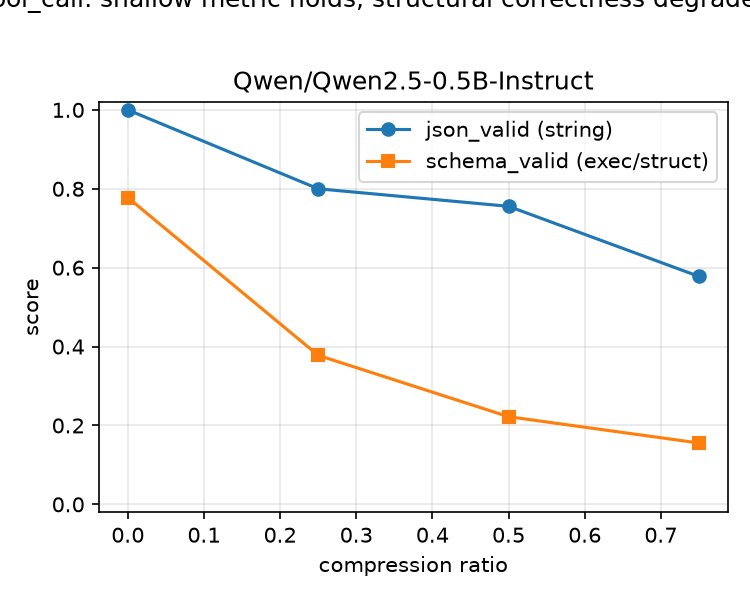
\includegraphics[width=0.65\linewidth]{figures/contrast_tool_call.png}
  \caption{\texttt{tool\_call} on Qwen2.5-0.5B-Instruct, averaged over the five presses. A shallow
  well-formedness check (\texttt{json\_valid}: did the model emit a parseable tool call?) stays high as
  the compression ratio rises, while \texttt{schema\_valid} (are the call's arguments actually valid
  for the tool?) collapses. A string-only or parse-only evaluation would report this regime as nearly
  lossless.}
  \label{fig:contrast}
\end{figure}

\subsection{tool\_call: well-formedness survives, correctness does not}

Figure~\ref{fig:contrast} shows the central result. Averaged over all five presses,
\texttt{json\_valid} retains $0.58$ of its uncompressed value at compression ratio $0.75$, while
\texttt{schema\_valid} retains only $0.20$. The model keeps producing things that parse as tool calls;
those calls are increasingly wrong.

The per-press breakdown (Table~\ref{tab:perpress}) is sharper. For the two best-behaved presses,
\texttt{Knorm} and \texttt{ExpectedAttention}, \texttt{json\_valid} never drops below $1.0$ at any
ratio: every output is a parseable tool call. Yet over the same ratios \texttt{schema\_valid} falls
from $0.78$ (uncompressed) to $0.33$, and the strictest metric \texttt{args\_exact} (exact argument
match, not shown) falls to $0$ for most presses by ratio $0.5$. A parse-rate metric would score these
presses at or near $100\%$ success precisely where a third to two-thirds of the tool calls have become
semantically invalid. \texttt{SnapKV} behaves similarly (\texttt{json\_valid} $\approx 1.0$,
\texttt{schema\_valid} $0.44 \to 0.11$). \texttt{StreamingLLM} collapses entirely on this model
(\texttt{json\_valid} $=0$ from ratio $0.25$), and \texttt{Random} degrades quickly as expected of a
floor; we report both rather than hide the outliers.

\begin{table}[t]
  \centering
  \small
  \begin{tabular}{lccccccc}
    \toprule
    & \multicolumn{4}{c}{\texttt{json\_valid} (shallow)} & \multicolumn{3}{c}{\texttt{schema\_valid} (correct)} \\
    \cmidrule(lr){2-5}\cmidrule(lr){6-8}
    press & base & 0.25 & 0.5 & 0.75 & 0.25 & 0.5 & 0.75 \\
    \midrule
    none              & 1.00 & --   & --   & --   & 0.78\,(base) & & \\
    Random            & 1.00 & 1.00 & 0.78 & 0.00 & 0.00 & 0.00 & 0.00 \\
    StreamingLLM      & 1.00 & 0.00 & 0.00 & 0.00 & 0.00 & 0.00 & 0.00 \\
    SnapKV            & 1.00 & 1.00 & 1.00 & 0.89 & 0.44 & 0.11 & 0.11 \\
    Knorm             & 1.00 & 1.00 & 1.00 & 1.00 & 0.89 & 0.67 & 0.33 \\
    ExpectedAttention & 1.00 & 1.00 & 1.00 & 1.00 & 0.56 & 0.33 & 0.33 \\
    \bottomrule
  \end{tabular}
  \caption{Per-press \texttt{tool\_call} on Qwen2.5-0.5B-Instruct. The uncompressed baseline is
  \texttt{json\_valid}$=1.00$, \texttt{schema\_valid}$=0.78$. For \texttt{Knorm} and
  \texttt{ExpectedAttention}, \texttt{json\_valid} stays at $1.00$ across all ratios while
  \texttt{schema\_valid} falls by half or more: well-formedness is preserved, correctness is not.}
  \label{tab:perpress}
\end{table}

\subsection{code\_exec at this scale}

On the ten-problem HumanEval slice, Qwen2.5-0.5B-Instruct scores \texttt{pass@1}$=0$ even uncompressed,
so compression cannot make it worse and the task yields no contrast at this model size (the string
anchor \texttt{edit\_sim} is likewise near zero, $\approx 0.08$, because the small instruct model
emits prose-wrapped rather than canonical completions). We report this honestly: the \texttt{code\_exec}
harness runs, executes, and scores correctly, but a 0.5B model on a CPU is too weak to produce a
meaningful executable-correctness signal. Demonstrating the \texttt{code\_exec} contrast requires a
capable code model on a GPU, which we leave as the immediate follow-up. The benchmark is released with
both tasks.

\section{Discussion and Limitations}
\label{sec:discussion}

\paragraph{Scale.} The headline limitation is scale: a single CPU box, small models, and a small
problem count. We therefore do not claim quantitative degradation rates for production-scale models;
we claim that the measurement gap is real and that the divergence appears even at this scale. The
harness is press- and model-agnostic, so reproducing at scale on a GPU is a configuration change.

\paragraph{Prefill-only regime.} We study prefill-time compression of a shared context. Decode-time
compression and per-request contexts are out of scope here.

\paragraph{Isolation.} \texttt{code\_exec} isolation is eval-grade, not adversarial; it should be run
on throwaway or CI hardware.

\paragraph{Threshold framing.} Where a structural metric holds at low ratios and falls at higher
ratios, the useful reading is a degradation \emph{onset}: the compression ratio at which functional
correctness departs from what string metrics would suggest.

\section{Conclusion}
\label{sec:conclusion}

KV-cache compression is validated with instruments that cannot see the damage it is most likely to
cause to structured generation. \texttt{kv-exec-bench} supplies the missing instruments, code pass@1
and tool-call schema validity, on top of \texttt{kvpress}. Even a small CPU-only study shows string
anchors holding while executable correctness drops. We hope the benchmark makes executable
correctness a routine axis when reporting KV-compression results.

\paragraph{Availability.} Code and benchmark: \url{https://github.com/pjdurden/kv-exec-bench} (Apache-2.0).

\bibliographystyle{plain}
\bibliography{refs}

\end{document}
